\section{Procedimento \& Analisi Dati}

Poichè stiamo lavorando in ambito di ottica geometrica e affinchè valgana la legge del costruttore di lenti e quella dei punti coniugati, dobbiamo fare alcune assunzioni relative all'apparato.
L'ipotesi fondamentale sulla quale si basa tutta l'esperieza e che i raggi luminosi incidenti sulle nostre lenti siano raggi parassiali, ovvero ci dobbiamo porre nell'ipotesi di raggi lontani.
Inoltre per non appesantire la lettura, nel seguito indicheremo con queste lettere le seguenti quantità:

%\begin{figure}[b!]
%	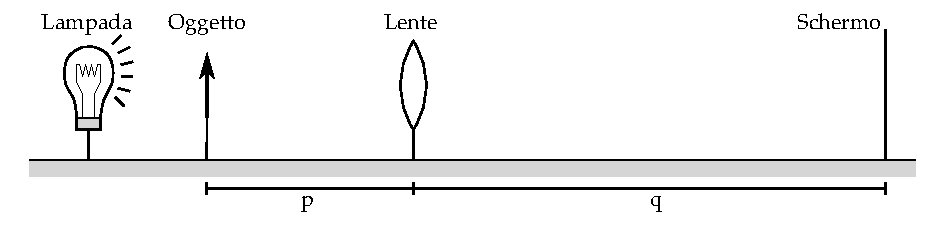
\includegraphics[width=16cm]{drawing.pdf}
%\end{figure}

\begin{equation*}
	p \,=\, \text{distanza tra il cento della lente e la posizione dell'oggetto}
\end{equation*}
\begin{equation*}
	q \,=\, \text{distanza tra il cento della lente e la posizione dell'immagine}
\end{equation*}
\begin{equation*}
	f \,=\, \text{fuoco della lente analizzata}
\end{equation*}
\begin{equation*}
	h \ped{imm} \,=\, \text{altezza dell'immagine sullo schermo}
\end{equation*}
\begin{equation}
	\text{Legge dei puni coniugati:} \qquad \frac{1}{f} \,=\, \frac{1}{p} + \frac{1}{q}
	\label{coniugati}
\end{equation}
\begin{equation}
	\text{Legge del costruttore di lenti:} \qquad \frac{1}{f} \,=\, (n-1)\left(\frac{1}{R\ped{1}}-\frac{1}{R\ped{2}}\right)
	\label{costruttore}
\end{equation}


\subsection{Fuoco della lente convergente}

Come primo obbiettivo ci siamo posti quello di calcolare il fuoco della lente convergente. Per ottenere questo riultato abbiamo misurato per dodici volte il valore che il parametro $q$ assume al variare del parametro $p$. Questo è stato fatto tenendo ferma la sorgente luminosa e incrementando di volta in volta la distanza tra la lente e la sorgente luminosa. Quindi abbiamo rilevato i valori di $q$ mettendo a fuoco l'immagine proiettata sullo schermo.

E' importante sottolineare che nel caso in cui l'immagine si è formata ad una grande distanza dalla lente, riuscire a metterla a fuoco non è stato semplice a causa dell'effetto di profondità di campo. Abbiamo deciso quindi di prendere due misure di $q$. Pertanto una volta che l'immagine ci sembrava essere a fuoco abbiamo mosso lo schermo in avanti e in dietro in modo da avere l'immagine leggermente fuori fuoco in entrambe le situazioni e abbiamo annotato le due posizioni. Facendone la media di questi due valori dovremmo ottenere un valore più probabile per la nostra variabile $q$, rispetto ad un singolo dato preso quando l'immagine è a ``fuoco''.

Una volta ottenuti i valori  di $p$ e $q$, abbiamo calcolato per ognuno il relativo valore di $f$ e infine ne abbiamo fatto una media.
Il valore ottenuto della focale $f$ della lente convergente è:

\begin{equation}
	f \ped{div} \,=\, XXX
\end{equation}

Inoltre vogliamo ricavare il valore della magnificazione per ogni coppia $p$ e $q$. Ricordiamo che la magnificazione è il rapporto tra le dimensioni dell'immagine ottenuta ($h \ped{imm}$) rispetto alle dimensioni reali dell'oggetto ($h$).

\begin{equation}
	m_{1} \,=\, \frac{h \ped{imm}}{h}
\end{equation}

Infine per avere una verifica della correttezza dei dati da noi presi possiamo mettere a confronto il valore della magnificazione trovato empiricamente con quello che si può ricavare dalla seguente relazione:

\begin{equation}
	m_{2} \,=\, \frac{q}{p}
\end{equation}

[Tabella m e m\']

Come si può osservare dai dati in tabella i due valori della magnificazione ricavati con entrambi i procedimenti risultano compatibili entro i propri errori. 

\subsection{Aberrazione cromatica relativa alla lente convergente}

Per valutare e osservare il fenomeno dell'aberrazione cromatica per la lente convergente abbiamo calcolato grazie alla relazione (\ref{coniugati}) il fuoco relativo ai raggi luminosi monocromatici rossi e blu. Per ottenere i raggi monocromatici non abbiamo fatto altro che porre un vetrino colorato difronte alla sorgente luminosa. I valori di $p$ e $q$ sono stati presi seguendo lo stesso procedimento adottato per la lente convergente, salvo il fatto che è stato preso solo un valore dei due parametri.
Un piccolo accorgimento che è stato preso nell'eseguire questa misura è stato quello di scegliere una distanza $p$ che fosse simile alla distanza $q$.
I risultati da noi ottenuti sono riportati nella tabella sottostante:

[TABELLA!!!]

Come si può notare dai dati in tabella i valori per il fuoco della lente convergente sono differerenti a seconda della lunghezza d'onda (colore) dei raggi luminosi incidenti su quest'ultima. 

\subsection{Aberrazione sferica relativa alla lente convergente}

Per descrivere questo fenomeno diamo un'idea di quello che si intende con:
\begin{itemize}
	\item{Fascio di luce cenrale: è l'insieme dei raggi luminosi che investono la lente convergente nel suo centro;}
	\item{Fascio di luce divergente: e l'insieme dei raggi luminosi che incidono sulla periferia della lente ovvero sulla sezione circolare, più distante dal centro, di quest'ultima;}
\end{itemize}
Adottato lo stesso accorgimento del punto precedente e fissata la distanza $p$ abbiamo esaminato il valore di $q$ selezionando solo il fascio di luce centrale. Questo è stato possibile perchè abbiamo posto sula lente un diaframma che ne oscurava tutta la superficie a parte la sezione centrale. Quindi si poteva supporre che i raggi incidenti formassero un angolo di $\frac{\pi}{2}$ con la superficie.
Successivamente per troare il valore di $q$ relativo al fascio di luce divergente abbiamo posto sulla lente un diaframma, ma con una fenditura circolare distante dal centro, in modo che i raggi incidenti sulla superficie non siano perpendicolari.
Quindi grazie ai valori di $q$ possiamo ora ricavare i valori della focale nei due casi. I isultati sono riportati nela tabella sottostante:

[TABELLA!!!]

Come si può notare per il facio di luce divergente il valore della focale della lene risulta essere minore rispetto al valore ottenuto per i raggi centrali. Questo succede proprio perchè nel secondo caso per i raggi luminosi non era più valida l'approssimazione di raggi parassiali.

\subsection{Fuoco della lente divergente}

Dal momento che per una lente divergente l'immagine che si ottiene è un immagine virtuale e non reale, ovvero l'immagine non si forma per intersezione dei raggi reali, ma per il loro prolungamento. Quindi risulterebbe impossibile misurare dirttamente il valre di $q$ usando solamente la lente divergente.
A tal fine abbiamo assemblato un sistema di lenti illustrato nella figura sottostante.

[STESSA FIGURA PRECEDENTE CON AGGIUNTA LA LENTE DIVERGENTE TRA LA SORENTE E LA LENTE DIVERGENTE]

Quindi indicando con:
\begin{itemize}
	\item{$p\ped{d}\,\,$ la distanza tra la sorgente luminosa e il centro della lente divergente;}
	\item{$D\,\,$ la distanza tra le due lenti;}
	\item{$q\ped{c}\,\,$ òa distanza tra il centro della lente convergente e l'immagine;}
	\item{$x\,\,$ la distnza incognita tra il centro della lente divergente e l'immagine data da questa;}
\end{itemize}
Il sistema ideato funziona nel seguente modo: la lente divergente produce un'mmagine virtuale tra la sorgente e se stessa. Qusta immagine diventa quindi il nuovo oggetto per la lente convergente che produce un immagine sullo schermo che noi possiamo vedere. Quindi potendo misurare tutti i parametri sopraelencati ad eccezzione di $x$ e $f\ped{d}$ (focale lente divergente) e conoscendo $f\ped{c}$ (focale lente convergente) risolvendo questo semplice sistema:

%\begin{equation}
%	\frac{1}{f\ped{d}} \,=\, \frac{1}{p\ped{d}} + \frac{1}{x}
%	\frac{1}{f\ped{c}} \,=\, \frac{1}{(D + x)} + \frac{1}{q\ped{c}}
%\end{equation}

\[ \left\{
  \begin{array}{l l}
    \frac{1}{f\ped{d}} \,=\, \frac{1}{p\ped{d}} + \frac{1}{x}\\
    \frac{1}{f\ped{c}} \,=\, \frac{1}{(D + x)} + \frac{1}{q\ped{c}}
  \end{array}
\right.\]
%
possiamo ottenere i valori di $x$ e $f\ped{d}$. Inoltre per ottenere un valore più accurato di $f\ped{d}$ abbiamo tenuta ferma la distanza $p\ped{d}$ e abbiamo variato la distanza $D$ e quindi anche $q\ped{c}$, per tre volte. Quindi per ognuna tripletta abbiamo sfruttato la relazione (\ref{coniugati}) e abbiamo ottenuto tre valori di $f\ped{d}$. facndomne pertanto la media otterremo un valore più ccurato di $f\ped{d]$
Quindi abbiamo ottenuto che:

\begin{equation}
	x \,=\, XXX \qquad \text{e} \qquad f\ped{d} \,=\, XXX
\end{equation}

\subsection{indice di rifrazione della lente convergente}

Per ricavare il valore dell'indice di rifrazione della lente convergente ($n$) non dobbiamo fare altro che sfruttare la relazione (\ref{costruttore}). A tal fine abbiamo usato il calibro per misurare i diametro della lente, il suo spessore al centro e quello al bordo. Tutti questi dati sono necessari in quanto nella legge sopracitata sono necessari i valori di $R\ped{1}$ e $R\ped{2}$ che nel nostro caso hanno valore uguale. $R\ped{1}$ e $R\ped{2}$ non sono altro che le distanze tra il centro della lente e la superficie della stessa. Quindi il problema di ricavare $R\ped{1}$ e $R\ped{2}$ si riduce ad un semplice problema di gometria elementare.
Il valore ottenuto di $R$ e: $R \,=\, XXX$.
Quindi per concludere il vaore dell'indice di rifrazione ($n$) della lente convergente risulta essere:

\begin{equation}
	n \,=\, XXX
\end{equation}







